% Modelo de Trabalho Acadêmico da UNESP de Guaratinguetá v-1.0
% Copyright 2017 by Eduardo Rohde Eras
%
% This program is free software: you can redistribute it and/or modify
% it under the terms of the GNU General Public License as published by
% the Free Software Foundation, either version 3 of the License, or
% (at your option) any later version.
%
% This program is distributed in the hope that it will be useful,
% but WITHOUT ANY WARRANTY; without even the implied warranty of
% MERCHANTABILITY or FITNESS FOR A PARTICULAR PURPOSE.  See the
% GNU General Public License for more details.
%
% You should have received a copy of the GNU General Public License
% along with this program.  If not, see <http://www.gnu.org/licenses/>.

%----------------------------------------------------------------------------------------%
% C L A S S E   D O   D O C U M E N T O
%----------------------------------------------------------------------------------------%

\documentclass[
  %----------------------------------------------------------------------------------------%
  %Opções da classe 'memoir'
  %----------------------------------------------------------------------------------------%
  12pt,		% Tamanho da Fonte.
  a4paper,	% Tamanho da página.
  openright,% Capítulos começam em páginas ímpares (insere uma página vazia se necessário).
  oneside,	% Para impressão em frente e verso utilizar twoside.
  %----------------------------------------------------------------------------------------%
  %Opções da classe 'abntex2'
  %----------------------------------------------------------------------------------------%
  chapter=TITLE,		%Títulos de capítulos convertidos em letras maiúsculas.
  section=TITLE,		%Títulos de seções convertidos em letras maiúsculas.
  %----------------------------------------------------------------------------------------%
  %Opções da classe 'babel'
  %----------------------------------------------------------------------------------------%
  english,	%Idioma adicional para hifenização.
  french,	%Idioma adicional para hifenização.
  spanish,	%Idioma adicional para hifenização.
  brazil	%Idioma principal do documento.
  %----------------------------------------------------------------------------------------%
]{abntex2}

%----------------------------------------------------------------------------------------%
% P A C O T E S
%
% Insira aqui os pacotes que for utilizar em seu documento. Para saber quais pacotes o
% template já está utilizando, confira o arquivo "pacoteBasico.sty".
%----------------------------------------------------------------------------------------%
    
    \usepackage{pacoteBasico}   %Pacote Básico de formatação no padrão da UNESP/FEG
    \usepackage{color}		    %Controle das cores.
    \usepackage{graphicx}	    %Inclusão de gráficos.
    \usepackage{lipsum}		    %Para geração de 'Dummy Text'.
    
%----------------------------------------------------------------------------------------%
% I N F O R M A Ç Õ E S   B Á S I C A S   S O B R E   O   T R A B A L H O
%
% Defina aqui as informações pertinentes ao trabalho.
%----------------------------------------------------------------------------------------%

    %----------------------------------------------------------------------------------------%
    % D A D O S   P E S S O A I S
    %----------------------------------------------------------------------------------------%
    
    %Nome completo do autor do presente Trabalho de Graduação:
    \newcommand{\nomeDoAutor}{
    Nome Completo do Autor
    }
    
    %Nome do curso em que o autor está se graduando:
    \newcommand{\nomeDoCurso}{
    Nome do Curso
    }
    
    %----------------------------------------------------------------------------------------%
    % D A D O S   S O B R E   O   T R A B A L H O
    %----------------------------------------------------------------------------------------%
    
    %Título do presente trabalho:
    \newcommand{\tituloDoTrabalho}{
    Título do Trabalho
    }
    
    %Subtítulo do presente trabalho, se houver:
    \newcommand{\subtituloDoTrabalho}{
    Subtítulo do Trabalho
    }
    
    %Mês da entrega do trabalho
    \newcommand{\mesDeEntrega}{
    Janeiro
    }
    
    %Ano da entrega do trabalho
    \newcommand{\anoDeEntrega}{
    2017
    }
    
    %----------------------------------------------------------------------------------------%
    % D A D O S   D O S   O R I E N T A D O R E S,   B A N C A   E   C O O R D E N A D O R
    %----------------------------------------------------------------------------------------%
    
    %Nome do orientador do presente trabalho:
    \newcommand{\nomeDoOrientador}{
    Nome Completo do Orientador
    }
    
    %Título do orientador:
    \newcommand{\tituloDoOrientador}{
    Profº Dr.
    }
    
    %Nome do coorientador do presente trabalho:
    \newcommand{\NomeDoCoorientador}{
    Nome Completo do Coorientador
    }
    
    %Título do coorientador:
    \newcommand{\tituloDoCoorientador}{
    Profº Dr.
    }
    
    %Nome do Coordenador do Curso:
    \newcommand{\nomeDoCoordenador}{
    Nome Completo do Coordenador
    }
    
    %Título do coordenador do Curso:
    \newcommand{\tituloDoCoordenador}{
    Profº Dr.
    }
    
    %Nome do Membro Interno da Banca:
    \newcommand{\nomeDoMembroInterno}{
    Nome Completo do Membro Interno
    }
    
    %Título do Membro Interno da Banca:
    \newcommand{\tituloDoMembroInterno}{
    Profº Dr.
    }
    
    %Nome do membro Externo da banca:
    \newcommand{\nomeDoMembroExterno}{
    Nome Completo do Membro Externo
    }
    
    %Título do Membro Externo da Banca:
    \newcommand{\tituloDoMembroExterno}{
    Profº Dr.
    }
    
    %----------------------------------------------------------------------------------------%
    % D A D O S   D A   I N S T I T U I Ç Ã O
    %----------------------------------------------------------------------------------------%
    
    %Nome da Universidade
    \newcommand{\nomeDaUniversidade}{
    Universidade Estadual Paulista "Júlio de Mesquita Filho"
    }
    
    %Nome da Cidade
    \newcommand{\nomeDaCidade}{
    Guaratinguetá
    }

%----------------------------------------------------------------------------------------%
% I N Í C I O   D O   D O C U M E N T O - P R É   T E X T U A L
%----------------------------------------------------------------------------------------%
\begin{document}
    
    \imprimircapa
    \imprimirfolhaderosto
    
    %------------------------------------------------------------------------------------%
    % F O L H A   D E   A P R O V A Ç Ã O
    %
    % OBRIGATÓRIO. Este é o modelo de folha de aprovação que deve ser digitalizada após as
    % assinaturas da banca. Utilize um software de edição de PDF para substituição posterior
    % dessa folha. Se possível, utilize um recurso de assinatura digital fornecido pela
    % ferramenta de edição de PDF, evitando assim a digitalização da folha toda.
    %------------------------------------------------------------------------------------%
    \begin{folhadeaprovacao}
        \begin{center}
        
        {\sffamily
            \bfseries{
                \Large{
                    UNIVERSIDADE ESTADUAL PAULISTA\par
                    "JÚLIO DE MESQUITA FILHO"\par
                }
            }
            CAMPUS DE GUARATINGUETÁ
        }
        
        \vspace*{3cm}
                
        \normalsize{\textbf{\MakeUppercase\nomeDoAutor}}
        
        \vspace*{1cm}
        
       % {\setstretch{1.0}
        \begin{framed}
            ESTE TRABALHO DE GRADUAÇÃO FOI JULGADO ADEQUADO COMO PARTE DO REQUISITO PARA A OBTENÇÃO DO DIPLOMA DE \textbf{"GRADUANDO EM {\MakeUppercase\nomeDoCurso}"}
            \par
            \vspace*{1cm}
            APROVADO EM SUA FORMA FINAL PELO CONSELHO DE CURSO DE GRADUAÇÃO EM {\MakeUppercase\nomeDoCurso}
            \par
            \vspace*{1cm}
            \begin{flushright}
            \tituloDoCoordenador {\MakeUppercase\nomeDoCoordenador}
            \par
            Coordenador
            \end{flushright}
       \end{framed}
      % }
       
       \begin{flushleft}
            \textbf{BANCA EXAMINADORA:}
       \end{flushleft}
       
       \assinatura{\small \tituloDoOrientador \nomeDoOrientador \par Orientador/UNESP-FEG}
       \assinatura{\small \tituloDoMembroInterno \nomeDoMembroInterno \par UNESP-FEG}
       \assinatura{\small \tituloDoMembroExterno \nomeDoMembroExterno \par Membro Externo}
       
       \vfill
       \mesDeEntrega, \anoDeEntrega
        
        \end{center}
    \end{folhadeaprovacao}
    
    %------------------------------------------------------------------------------------%
    % D A D O S   C U R R I C U L A R E S
    % 
    % OBRIGATÓRIO PARA PÓS-GRADUAÇÃO.
    % Inserir a data inicial e final de cada formação acadêmica. Para os alunos que não
    % precisarem de uma folha de dados curriculares em seu trabalho, basta apagar todo 
    % o código dessa seção.
    %------------------------------------------------------------------------------------%
    
    \begin{center}
        \normalsize{\textbf{\MakeUppercase{Dados Curriculares}}} \par
        \vspace*{1cm}
        \normalsize{\textbf{\MakeUppercase\nomeDoAutor}} \par
        \vspace*{1cm}
        
        \begin{tabular}{ l p{7cm} }
            \textbf{\MakeUppercase{Nascimento}} & Data - Cidade / Sigla do Estado \\
            \\
            \textbf{\MakeUppercase{Filiação}} & Nome completo do Pai \\
            & Nome completo da Mãe \\
            \\
            \textbf{\MakeUppercase{Ano Inicial / Ano Final}} & Formação acadêmica ou Complementar (nome do curso e titulação) \\
            & Instituição de Ensino \\
            \\
            \textbf{\MakeUppercase{Ano Inicial / Ano Final}} & Formação acadêmica ou Complementar (nome do curso e titulação) \\
            & Instituição de Ensino \\
            \\
            \textbf{\MakeUppercase{Ano Inicial / Ano Final}} & Formação acadêmica ou Complementar (nome do curso e titulação) \\
            & Instituição de Ensino \\
        \end{tabular}
    \end{center}
    \newpage
    
    %------------------------------------------------------------------------------------%
    % D E D I C A T Ó R I A
    %
    % OPCIONAL. Se não for utilizar uma dedicatória, basta apagar todo o código dessa seção.
    %------------------------------------------------------------------------------------%
    
    \begin{dedicatoria}
        \vspace*{\fill}
        \begin{flushright}
            Sua dedicatoria deve ser digitada aqui.
        \end{flushright}
        \vspace*{1cm}
    \end{dedicatoria}

    %------------------------------------------------------------------------------------%
    % A G R A D E C I M E N T O S
    %
    % OPCIONAL. Citar as pessoas, instituição, agência de fomento, entre outros que contribuíram
    % de maneira relevante à elaboração do trabalho e na vida acadêmica.
    % Se não for utilizar os agradecimentos, basta apagar todo o código dessa seção.
    %------------------------------------------------------------------------------------%
    \begin{agradecimentos}
    
        Esse é um espaço reservado para os agradecimentos. Uma nota de rodapé\footnote{Essa é uma nota de rodapé} pode ser inserida desta forma para indicar alguma URL\footnote{\url{http:\\www.url.com.br}} que referencia o alvo de seu agradecimento.
    
    \end{agradecimentos}
    
    %------------------------------------------------------------------------------------%
    % F O M E N T O
    %
    % OBRIGATÓRIO PARA ALUNO BOLSISTA. Esta página contém informações sobre o financiamento
    % recebido para o desenvolvimento da tese/dissertação. Utilize o(s) nome(s) da(s) 
    % instituição(ões) que forneceu(ram) o auxílio financeiro para seu trabalho. Se não
    % for utilizar o fomento em seu trabalho, basta apagar todo o código dessa seção.
    %------------------------------------------------------------------------------------%
    \vspace*{\fill}
    \begin{flushleft}
        Este trabalho contou com o apoio da(s) seguinte(s) entidade(s):\\
        FAPESP - Fundação de Amparo à Pesquisa do Estado de São Paulo\\
        CAPES - Coordenação de Aperfeiçoamento de Pessoa de Nível Superior\\
        CNPq - Conselho Nacional de Desenvolvimento Científico e Tecnológico\\
        SIGQ - Sigla de Uma Instituição Genérica Qualquer
    \end{flushleft}
    \newpage
    
    %------------------------------------------------------------------------------------%
    % E P Í G R A F E
    %
    % OPCIONAL. Texto em que o autor apresenta uma citação, seguida de indicação de autoria.
    % Se não for utilizar uma epígrafe, basta apagar todo o código dessa seção.
    %------------------------------------------------------------------------------------%
    
    \begin{epigrafe}
        \vspace*{\fill}
    	\begin{flushright}
    		\textit{
        		``Frase, citação, epígrafe.``\\
        		(Autor)
    		}
    	\end{flushright}
    \end{epigrafe}
    
    %------------------------------------------------------------------------------------%
    % R E S U M O   N O   I D I O M A   D O   T E X T O
    %
    % OBRIGATÓRIO. Deve ser redigido em um só parágrafo contendo de 150 a 500 palavras e 
    % ressaltar: objetivo, método, resultados e as principais conclusões.
    % Após o resumo, são listadas palavras-chave relacionadas à temática do trabalho, 
    % separadas entre si por ponto e também finalizadas por ponto.  (NBR 6028, 2003)
    %------------------------------------------------------------------------------------%
    
    \begin{resumo}
    
        \lipsum[1] % Digite seu resumo no lugar deste comando.
        
        \vspace*{0.5cm}
    
        \noindent\textbf{\MakeUppercase{Palavras-Chave: }} palavra-chave. palavra-chave. palavra-chave.
    
    \end{resumo}
    
    %------------------------------------------------------------------------------------%
    % A B S T R A C T :   R E S U M O   N O   I D I O M A   E S T R A N G E I R O
    %
    % OBRIGATÓRIO. Elaborado com as mesmas características do resumo em língua portuguesa.
    % Se redigido em inglês-ABSTRACT, em castelhano-RESUMEN, em francês-RÉSUMÉ.
    % Após o resumo, são listadas palavras-chave relacionadas à temática do trabalho no 
    % idioma escolhido. Se redigido em inglês - KEYWORDS, em espanhol - PALABRAS CLAVES,
    % em francês - MOTS-CLÉS.
    %------------------------------------------------------------------------------------%
    
    \begin{resumo}[Abstract] % Substitua 'Abstract' pela palavra no idioma desejado, caso precise.
    
        \lipsum[1] % Digite seu abstract no lugar deste comando.
        
        \vspace*{0.5cm}
        
        %Subistitua 'Keywords' pela palavra no idioma desejado, caso precise.
        \noindent\textbf{\MakeUppercase{Keywords: }} keyword. keyword. keyword.
    
    \end{resumo}
    
    %------------------------------------------------------------------------------------%
    % L I S T A   D E   I L U S T R A Ç Õ E S
    %
    % OPCIONAL. Quando necessário recomenda-se a elaboração de lista própria para cada tipo
    % de ilustração (figuras, fotografias, organogramas, quadros, etc).(NBR14724, 2011)
    % Se não for utilizar uma Lista de Ilustrações, basta apagar todo o código dessa seção.
    %------------------------------------------------------------------------------------%
    
    \listoffigures*
    \newpage
    
    %------------------------------------------------------------------------------------%
    % L I S T A   D E   T A B E L A S
    %
    % OPCIONAL. Se não for utilizar uma Lista de Tabelas, basta apagar todo o código
    % dessa seção.
    %------------------------------------------------------------------------------------%
    
    \listoftables*
    \newpage
    
    %------------------------------------------------------------------------------------%
    % L I S T A   D E   A B R E V I A T U R A S   E   S I G L A S
    %
    % OPCIONAL. Consiste na relação alfabética das abreviaturas e siglas utilizadas,
    % seguidas das palavras ou expressões correspondentes escritas por extenso.
    % Se não for utilizar uma Lista de Abreviaturas, basta apagar todo o código dessa seção.
    %------------------------------------------------------------------------------------%
    
    \begin{siglas}
        \item[TCC] Trabalho de Conclusão de Curso
        \item[UNESP] Universidade Estadual Paulista
    \end{siglas}
    
    %------------------------------------------------------------------------------------%
    % L I S T A   D E   S Í M B O L O S
    %
    % OPCIONAL. Os símbolos devem ser listados de acordo com a ordem apresentada no texto,
    % com seus respectivos significados. Se não for utilizar uma Lista de Símbolos, basta
    % apagar todo o código dessa seção.
    %------------------------------------------------------------------------------------%
    
    \begin{simbolos}
        \item[$\alpha$] Letra Grega Alfa
        \item[$\beta$] Letra grega Beta
        \item[$\gamma$] Letra grega Gama
        \item[$e$] Número de Euler
        \item[R\$] Unidade monetária Brasileira (Real)
    \end{simbolos}
    
    %------------------------------------------------------------------------------------%
    % S U M Á R I O
    %
    % OBRIGATÓRIO. Havendo mais de um volume, cada um deve conter o sumário completo do
    % trabalho (NBR6024; NBR6027, 2012). Não se deve confundir sumário com índice.
    %------------------------------------------------------------------------------------%
    
    \tableofcontents*
    \newpage
    
    %------------------------------------------------------------------------------------%
    %                                                                                    %
    %                           C O R P O   D O   T E X T O                              %
    %                                                                                    %
    %                     Seu trabalho começa a ser digitado aqui.                       %
    %                                                                                    %
    % Início do corpo do texto. A partir desse comando será impresso o número de páginas.%
    %------------------------------------------------------------------------------------%
    
    \textual
    \pagestyle{simple} 
    
    %------------------------------------------------------------------------------------%
    
    \chapter{Introdução}
    
    Será abordado no corpo do texto desse template um guia de como redigir seu trabalho utilizando as Diretrizes da Biblioteca, que podem ser consultadas pelo site: \url{http://www2.feg.unesp.br/Home/Biblioteca21/diretrizes-2016.pdf}. É muito importante a leitura desse guia para elaboração de seu documento \LaTeX: Serão apresentados exemplos de citações, formatações de tabelas e figuras, estrutura de níveis de seção, formulas matemáticas, entre outros. É aconselhável não apagar essas dicas de seu documento durante a elaboração do seu trabalho! Utilize esse texto como guia durante toda elaboração de seu documento.
    
    \chapter{Desenvolvimento}
    
        Vamos mostrar aqui alguns exemplos de citações e ilustrações que podem ser utilizadas no texto.
        
        \section{CITAÇÕES}
        
            Uma citação \cite{carbono} simples é dada pelo comando \verb|\cite{}|, referenciando uma entrada no arquivo \verb|references.bib|. As citações podem referenciar diferentes tipos de documentos. Esse é um exemplo de uma citação de um livro \cite{livro}. Esse é um exemplo de uma citação de artigo \cite{artigo}. Esse é um exemplo de uma citação de um site \cite{website}.
        
        \section{CITAÇÃO DIRETA}
        
            Citações diretas com até três linhas, deve ser destacada por aspas duplas. Para realizar citações diretas ou indiretas deve ser seguida a norma NBR 10520, 2002. "Este é um exemplo de citação direta com menos de três linhas."\cite{artigo}.
    
             Uma citação direta com mais de três linhas deve ser destacada com letra menor que o texto, espaço simples entrelinhas, recuo de 4 cm e separada por espaços de 1,5 (branco) antes e depois do texto. Abaixo, vemos um exemplo de como fazer uma citação direta:
            
            \vspace{1.5pt}
            \begin{flushright}
                \begin{minipage}{.724\textwidth}
                    {\SingleSpacing\small
                    Esse é um exemplo de citação direta com mais de três linhas. Ele será formatado conforme pedido, em um bloco separado de texto alinhado à direita da página com uma fonte de tamanho menor. É importante lembrar que ao final da citação devemos obrigatoriamente informar a referência. \cite[p.~3--4]{livro}
                    }
                \end{minipage}
            \end{flushright}
            \vspace{1.5pt}
             
             Utilize esse código toda a vez que for fazer uma citação direta com mais de 3 linhas. Mantenha todos os valores de alinhamento conforme o exemplo, substitua somente o conteúdo do texto pelo texto que irá utilizar.
             
        \section{CITAÇÃO INDIRETA}
        
            É a transcrição livre das ideias do autor citado. Na citação indireta a indicação da página é opcional. Em caso de dúvidas consulte as Diretrizes da Biblioteca disponíveis no site: \url{http://www2.feg.unesp.br/Home/Biblioteca21/diretrizes-2016.pdf}. Abaixo, vemos um exemplo de citação indireta:
            
            Segundo um Autor Exemplo \cite{livro}, esse é um exemplo de citação indireta, transcrita livremente da original, sem necessidade de mudar o tamanho da fonte.
            
            Note que a citação indireta tem sua referência citada logo no começo do parágrafo, e não ao final como na citação direta.
            
        \section{CITAÇÃO DE CITAÇÃO}
            
            É a citação direta ou indireta de um texto em que não se teve acesso ao original. Deve ser indicada pelo sobrenome do autor do documento original, seguido da expressão latina \textit{apud} (citado por, conforme, segundo) e dados da obra consultada. A seguir um exemplo de uma citação de citação:
            
            Para o Autor Exemplo \apud[p.~1--5]{website}{invisivel}, é possível citar uma citação feita por outro autor em seu documento \LaTeX.\footnote{SITE, A. do. \textbf{Título do Site}. 2017. Disponível em: \url{http://www.url.com} apud INVISÍVEL, \textbf{Obra Não Citada na Bibliografia}. Cidade, Editora Invisível, 2017}
            
            A referência deve ser feita em Nota de Rodapé (digitada manualmente, conforme o exemplo, em um comando \verb|\footnote{}|) e não incluída na lista de Referências. Portanto, o autor citado indiretamente deve estar marcado como \verb|@hidden| no arquivo \verb|.bib|. 
             
        \section{FIGURAS, TABELAS E QUADROS}
        
            Vamos mostrar aqui três exemplos: uma figura, uma tabela e um quadro, conforme devem ser exibidas no texto. Existem muitas formas diferentes de formatar um elemento utilizando os recursos do \LaTeX, o importante é manter a descrição, a referência e a formatação do elemento gráfico conforme o padrão.
            
            \subsection {Tabelas}
                Uma tabela expõe dados estatísticos, representados numericamente. A forma de apresentação é a seguinte: 
                \begin{itemize}
                    \item lados esquerdo e direito da tabela sempre abertos;
                    \item partes superior e inferior sempre fechadas;
                    \item não há traços horizontais e verticais para separar números, em seu interior.
                \end{itemize}
                
                Observação: Devem conter a fonte mesmo que elaborada pelo autor.
                
                \begin{table}[h]
                    \centering
                    \caption{Elementos Aleatórios}
                    \begin{tabular}{ccc}
                        \hline
                        \multicolumn{1}{|c|}{Elemento} & \multicolumn{1}{c|}{Tamanho} & \multicolumn{1}{c|}{Número}\\
                        \hline
                        He & pequeno & 2 \\
                        Pb & grande & 82 \\
                        \hline
                    \end{tabular}
                    \par
                    {\small fonte: Produção do Próprio Autor.}
                \end{table}
            
            \subsection {Quadros}
                
                Um quadro, como por exemplo o \ref{quadroUm} expõe informações qualitativas, geralmente representadas na forma de texto. Um quadro apresenta:
                
                \begin{itemize}
                    \item os quatro lados fechados;
                    \item traços horizontais e verticais;
                    \item identificação (Título) localizada na parte superior.
                \end{itemize}
                
                Um quadro é declarado dentro de um ambiente \verb|quadro| que foi especialmente criado para esse template, definido no arquivo \verb|pacoteBasico.sty|. Dentro desse ambiente é criado uma tabela (ambiente \verb|tabular|). Por padrão, todos os quadros serão listados na lista de figuras.

                \begin{quadro}[h]
                    \centering
                    \caption{Tipos de documentos acadêmicos}
                    \label{quadroUm}
                    \begin{tabular}{|l|p{12cm}|}
                    \hline
                    Documento & Caracterização \\ \hline
                    Monografia  & Similares (trabalho de conclusão de curso de graduação, monografia de curso de especialização e/ou aperfeiçoamento e outros): Documento que representa o resultado de estudo, devendo expressar conhecimento do assunto escolhido, que deve ser obrigatoriamente emanado da disciplina, módulo, estudo independente, curso, programa e outros ministrados. Deve ser feito sob a coordenação de um orientador. \\ \hline
                    Dissertação & Documento que representa o resultado de um trabalho experimental ou exposição de um estudo científico retrospectivo, de tema único e bem delimitado em sua extensão, com o objetivo de reunir, analisar e interpretar informações. Deve evidenciar o conhecimento da literatura existente sobre o assunto e a capacidade de sistematização do candidato. É feito sob a coordenação de um orientador (doutor), visando a obtenção do título de Mestre. \\ \hline
                    Tese & Documento que representa o resultado de um trabalho experimental ou exposição de um estudo científico de tema único e bem delimitado. Deve ser elaborado com base em investigação original, constituindo-se em real contribuição para a especialidade em questão. É feito sob a coordenação de um orientador (doutor), visando a obtenção do título de doutor ou similar. \\ \hline
                    \end{tabular}
                    \par
                    {\small fonte: Adaptado da NBR 14724 (2011)}
                \end{quadro}

            \subsection {Figuras}
            
                Qualquer que seja o tipo de ilustração (figuras, desenhos, gráficos, diagramas, fluxogramas, fotografias, mapa, planta, quadro, imagem entre outros) sua identificação (título) aparece na parte superior
                
                \begin{figure}[h]
                    \centering
                    \caption{Um livro}
                    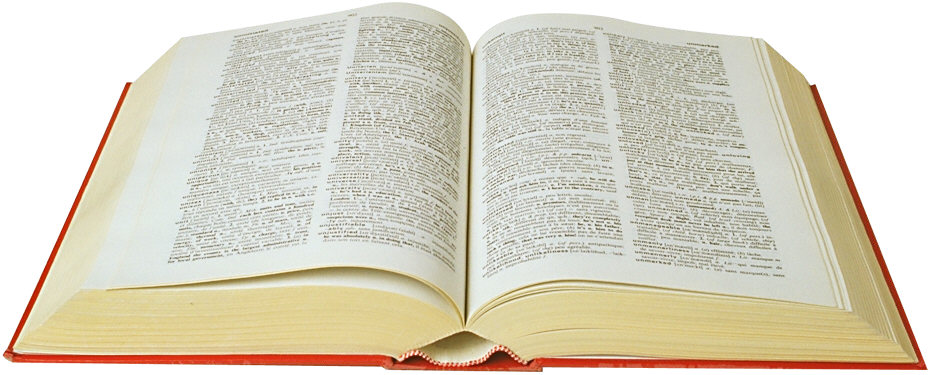
\includegraphics{book}
                    \par
                    {\small fonte: Produção do próprio autor.}
                \end{figure}
    
    \chapter {Equações}
        
        Fórmulas e Equações devem ser destacadas no texto de modo a facilitar sua leitura, sendo numeradas consecutivamente com algarismos arábicos entre parênteses. Fórmulas simples podem aparecer no próprio texto, sem necessidade de numeração.
        
        A equação \ref{eq:integral} de uma equação matemática destacada do texto. É de suma importância indicar o uso do ambiente \verb|equation|, que oferece uma melhor compatibilidade, maior flexibilidade além de referências cruzadas. O ambiente matemático indicado pelos símbolos "\$\$" deve ser evitado para qualquer expressão matemática destacada, sendo utilizado somente em uma expressão matemática simples que aparece junto ao texto.
        
        \begin{equation}
            \label{eq:integral}
            \int\limits_a^b f(x) dx = \lim_{x \to \infty} \displaystyle\sum_{i=1}^{n} f(x_i) \Delta i
        \end{equation}

        Uma expressão matemática simples pode ser incluída no corpo do texto. Por exemplo, o triângulo $a^2 = b^2 + c^2$ pode ser escrito utilizando o símbolo "\$" sem problemas. Qualquer expressão matemática pode ser incluída no corpo do texto para elaboração de um raciocínio. Mas toda expressão que se deseja destacar do texto deve ser redigida dentro do ambiente \verb|equation|.
    
    \chapter {Exemplo de Níveis de Seção}
    
        Nesse capítulo será ilustrado como se utilizar os diferentes níveis e subníveis de seção em seu documento. Estar atento quanto a identação do código para manter a clareza e organização de seu trabalho.
        
            \section{SEÇÃO EXEMPLO UM}
            Todo título de seção (primeiro nível abaixo do capítulo) deve ser escrita OBRIGATORIAMENTE com letras maiúsculas, dessa forma é garantido que o título de sua seção irá aparecer com letras maiúsculas no Sumário. Todas as demais subseções ou capítulos terão seus títulos formatados automaticamente no Sumário.
            
            \section{SEÇÃO EXEMPLO DOIS}
            Novamente, todo título de seção (primeiro nível abaixo do capítulo) deve ser escrita OBRIGATORIAMENTE com letras maiúsculas. Esse padrão deve ser mantido em todo texto.
            
                \subsection{Subseção Exemplo Um}
                \lipsum[8]
                
                \subsection{Subseção Exemplo Dois}
                \lipsum[7]
                
                    \subsubsection{Sub - Subseção Exemplo Um}
                    \lipsum[6]
                    
                    \subsubsection{Sub - Subseção Exemplo Dois}
                    \lipsum[12]
                    
                        \paragraph{Sub - Sub - Subseção Exemplo Um}
                        \lipsum[11]
                        
                        \paragraph{Sub - Sub - Subseção Exemplo Dois}
                        \lipsum[13]

    \chapter{Conclusão}
    
        Deve ser fundamentada no texto, contendo deduções lógicas e correspondentes aos objetivos propostos.
    
    %------------------------------------------------------------------------------------%
    %                               P Ó S   T E X T U A L                                %
    %                                                                                    %
    % Fim do corpo do texto. A partir desse comando as indicações no sumário serão       %
    % marcadas como 'pós textuais'.                                                      %
    %------------------------------------------------------------------------------------%
    
    \postextual
    
    %------------------------------------------------------------------------------------%
    % R E F E R Ê N C I A S
    %
    % OBRIGATÓRIO. Será gerada automaticamente a partir do arquivo "references.bib".
    %------------------------------------------------------------------------------------%
    
    \bibliography{references}
    
    %------------------------------------------------------------------------------------%
    % A P Ê N D I C E S
    %
    % OPCIONAL. Consiste em um texto ou documento elaborado pelo autor a fim de complementar
    % sua argumentação. Se necessário ter mais de um apêndice, basta adicionar cada um dentro
    % de um dentro de um comando "\chapter". % Se não for utilizar um Apêndice, basta apagar
    % todo o código dessa seção.
    %------------------------------------------------------------------------------------%
    
    \begin{apendicesenv}
        
        \chapter{Título do Apêndice A}
            \lipsum[50]
        
        \chapter{Título do Apêndice B}
            \lipsum[51]
        
    \end{apendicesenv}
    
    %------------------------------------------------------------------------------------%
    % A N E X O S
    %
    % OPCIONAL. Consiste em um texto ou documento não elaborado pelo autor que serve de
    % fundamentação, comprovação ou ilustração ao trabalho. Se necessário ter mais de um
    % anexo, basta adicionar cada um dentro de um dentro de um comando "\chapter".
    % Se não for utilizar nenhum Anexo, basta apagar todo o código dessa seção.
    %------------------------------------------------------------------------------------%
    
    \begin{anexosenv}
    
        \chapter{Título do Anexo A}
            \lipsum[30]
      
        \chapter{Título do Anexo B}
            \lipsum[31]
        
        \chapter{Título do Anexo C}
            \lipsum[32]
      
    \end{anexosenv}
    
\end{document}

